\documentclass[a4paper,12pt]{article}
\usepackage{blindtext}
\usepackage[utf8]{inputenc}
\usepackage{graphicx}
\usepackage{enumitem}
\usepackage{booktabs}
\usepackage{verbatim}
\usepackage{makecell}

\begin{document}
\begin{titlepage}
\center

\textsc{\LARGE User Manual}\\[1.5cm]
\textsc{\Large Project: Traffic Camera Image Analysis}\\[1.5cm]
\textsc{\large Client: DPSS, CSIR}\\[0.5cm]
\textsc{\large Team: Quadcore Productions}\\[0.5cm]

\begin{minipage}{0.4\textwidth}
\begin{flushleft} \large
\textbf{Author(s):}\\
Mpho \textsc{Baloyi}\\
Hlengekile \textsc{Jita}\\
Mayimela \textsc{Moses}\\
Mbhele \textsc{Themba}\\
\end{flushleft}
\end{minipage}
~
\begin{minipage}{0.4\textwidth}
\begin{flushright} \large
\textbf{Student number(s):} \\
14133670\\ % Student number
14077893\\
14019702\\
14007950\\
\end{flushright}
\end{minipage}\\

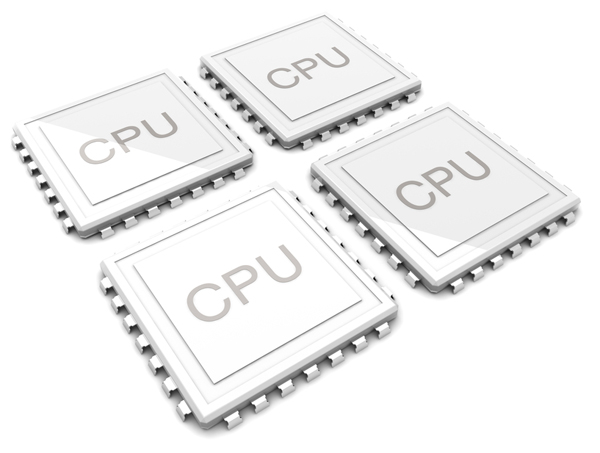
\includegraphics[width=\textwidth]{2012-quad-core-phones.jpg}

{\large University of Pretoria, Department of Computer Science}\\

{\large 29 July 2016}\\[3cm]

\vfil

\end{titlepage}

\newpage
\tableofcontents
\newpage

\newpage
%\begin{comment}
\begin{table}[ht]
 \centering
 \caption{Version History}
 \label{tab:table1}
 \begin{tabular}{cccc}
   \toprule
    Version No. & Date & Changes & By\\
    \midrule
    1 & 29 July 2016 & \makecell{Application Installation, \\ Application Use} & \makecell{Mpho Baloyi,\\ Hlengekile Jita,\\ Moses Mayimela,\\ Themba Mbhele} \\
    \bottomrule
  \end{tabular}
\end{table}
%\end{comment}
\newpage

\section{Application Installation}
In order to install this application you will need the following:
\begin{itemize}
\item An Android Device
\item The Traffic Camera Image Analysis system APK file
\end{itemize}

The Traffic Camera Image Analysis System .apk can be installed as follows:
\begin{enumerate}
\item \textbf{Make sure that third party apps are allowed on your device -} Go to Menu, then go to Settings, then go to Security and check the Unknown Sources option. This allow allow applications which aren't from the play store to be installed.
\item \textbf{Place the APK file in your device} 
\item \textbf{Install the application -} Select the APK file and it will install on your device
\end{enumerate}

\section{Application Use}
\subsubsection{Adding a Route}
The process of adding a route is as follows:
\begin{itemize}
    \item On the application bar which is located at the top of the screen, click on the menu button which is the button that contains three horizontal strips.
    \item A navigation drawer(menu) will then appear. On this menu, there will be a number of options. One of the options will be "Add Route". Click on this option to add a route.
    \item Once the above step has been executed, two input fields will be displayed  where you can enter a start location and an end location. Once they have been entered, you then press the send button and a route will be set up
\end{itemize}
\subsubsection{Modifying a Route}
\begin{itemize}
    \item On the application bar which is located at the top of the screen, click on the menu button which is the button that contains three horizontal strips.
    \item A navigation drawer(menu) will then appear. On this menu, there will be a number of options. One of the options will be "Modify Route". Click on this option to modify a route.
    \item Once the above step has been executed, two input fields will be displayed  where you can modify either the start location or end location, or both. Once they have been entered, you then press the send button and the route will be modified.
\end{itemize}
\subsubsection{Delete a Route}
\begin{itemize}
    \item On the application bar which is located at the top of the screen, click on the menu button which is the button that contains three horizontal strips.
    \item A navigation drawer(menu) will then appear. On this menu, there will be a number of options. One of the options will be "Delete Route". Click on this option to delete the currently selected route.
\end{itemize}
\end{document}